\chapter{Signale}
Zum Verständnis der Signalverarbeitung ist es notwendig eine
mathematische Beschreibung von Signalen zu entwickeln.
Da Signale sehr unterschiedlicher Natur sein können, werden wir zunächst eine grobe
Klassifikation vornehmen.

Um die einzelnen Signalklassen zu entwickeln, betrachten wir
einige Beispiele für natürliche Signale:

\begin{itemize}
    \item Sprache: Für den Studiengang H+A das Signal, das wir am besten
    kennen lernen sollten.
\begin{figure}[H]
\begin{center}
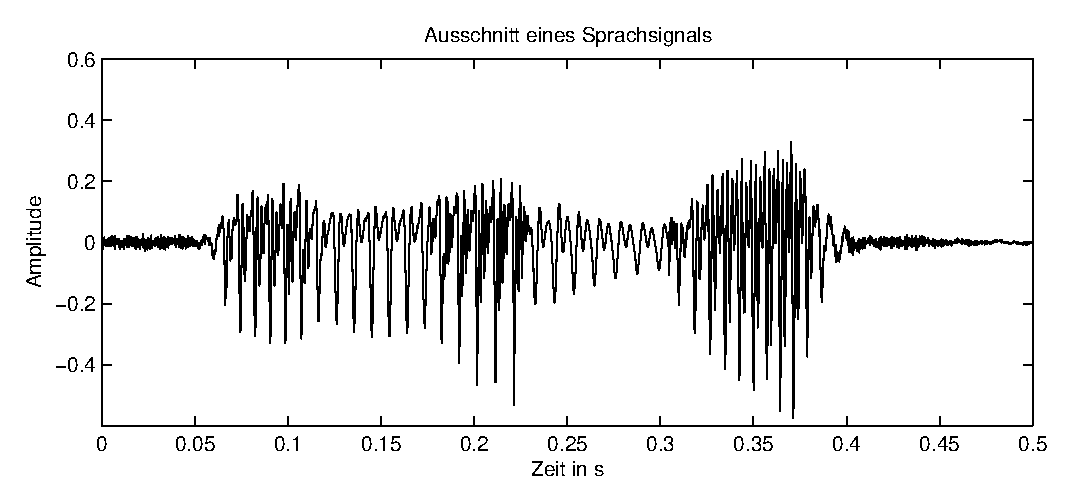
\includegraphics[width = 15cm]{ps/Sprachsignal}
\caption{\label{pic:Sprachsignal} Typischer Amplitidenverlauf über
der Zeit eines Sprachsignals.}
\end{center}
\end{figure}

    \item Musik: Ebenfalls für H+A sehr relevant.
    \item EKG und EEG- Signale (für AT und H+A relevant)
    \item Vitaldaten (Puls, Blutdruck)
    \item Bilder / Videos
    \item Radio- und Fernsehsignale
\end{itemize}

Aber auch aus völlig anderen Bereichen, lasen sich bestimmte
Größen als Signale interpretieren.
\begin{itemize}
    \item DAX-Abschlusskurse
\begin{figure}[H]
\begin{center}
\includegraphics[width = 7cm]{ps/BeispielDaxkurs}
\caption{\label{pic:Daxkurs} Verlauf des DAX bei einer Aktualisierung alle zwei Stunden.}
\end{center}
\end{figure}

    \item Verkehrsampelsignale

\begin{figure}[H]
\begin{center}
\includegraphics[width = 9cm]{ps/Verkehrsampelsignal}
\caption{\label{pic:Verkehrsampel} Ampelsignal im normalen Betrieb.}
\end{center}
\end{figure}

\end{itemize}

Mehr technischer Natur sind \zB
\begin{itemize}
    \item Das optische Signal, dass ein CD-Player von der CD liest
    \item Das Signal, dass ein Pulsmessgerät ausgibt.
    \item Ihr Beispiel
\end{itemize}

Als Gemeinsamkeiten fallen auf, dass die jeweiligen Signale meistens eine
unabhängige Größe beinhalten (meistens die Zeit) und eine abhängige Größe, zum Beispiel
den Schalldruck am Mund. Dies wird mathematisch durch $p(t)$ ausgedrückt\footnote{Aus
der Mathematik ist die Kurzform $y = x^2$ geläufiger als $y(x) = x^2$.}.
Weiterhin ist allen Signalen gemeinsam, dass sie
eine bestimmte Information enthalten.
Deshalb definieren wir:
\wichtig{Signale sind Funktionen oder Wertfolgen, die Informationen repräsentieren}

\section{Klassifikation}
Wir haben gesehen, dass es viele unterschiedliche Signalarten gibt. Die Frage, die sich
stellt ist, ob es Gemeinsamkeiten zwischen verschiedenen Signalen gibt und
wie wir diese Gemeinsamkeiten bezeichnen. Dies kann grob als eine Art Klassifikation der
Signale betrachtet werden.

\subsection{Wertebereich}
Eine erste Unterteilung ist möglich, indem wir den Wertebereich der unterschiedlichen
Signale untersuchen. Es fällt auf, dass ein Teil der Signale keinerlei Grenzen
in der Auflösung haben, so ist bei natürlich gesprochener Sprache, jeder Schalldruck
innerhalb der physikalischen Grenzen
möglich. Im Gegensatz dazu nimmt eine Ampel im Normalbetrieb nur vier Zustände an.

Dies führt zu der Kategorie Wertebereich, die in die beiden Klassen
\wichtig{wertkontinuierlich vs. wertdiskret}
unterteilt werden kann.

\subsection{Definitionsbereich}
Eine weitere sehr wichtige Unterteilung ist der Definitionsbereich. Für Signale
ist dies die Frage der Gültigkeit eines Signals. Beim natürlichen Sprachsignal ist die Gültigkeit
immer gegeben. Ein Gegenbeispiel ist der DAX-Abschlusskurs, der immer nur
um 20.00 Uhr gültig ist.

Somit können wir eine weitere Unterteilung definieren.
\wichtig{zeitkontinuierlich vs. zeitdiskret}

Nur wenn ein Signal in den beiden Kategorien diskret ist, spricht man von einem {\bf digitalen Signal}.

\wichtig{Ein digitales Signal ist wert- und zeitdiskret.}

Abbildung \ref{pic:TabelleWertZeit} zeigt die vier
Kombinationsmöglichkeiten, die sich durch die beiden Kategorien
Wertebereich und Definitionsbereich ergeben.

\begin{figure}[H]
\begin{center}
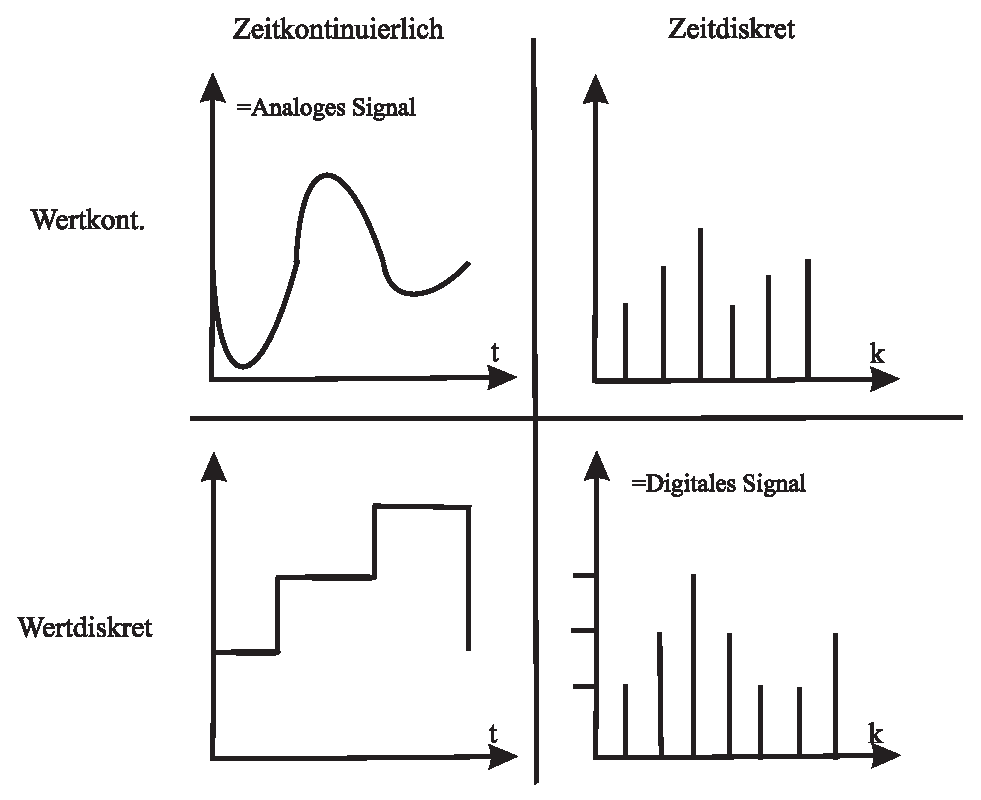
\includegraphics[width = 14cm]{ps/TabelleWertZeit}
\caption{\label{pic:TabelleWertZeit} Die vier
Kombinationsmöglichkeiten für wert- oder zeitkontinuierliche bzw.
wert- oder zeitdiskrete Signale.}
\end{center}
\end{figure}

\subsection{Kanalanzahl}
Betrachtet man die genannten Beispiele, so fällt zumindest bei der CD auf, dass
das Ausgabesignal zweikanalig ist, um die Stereophonie zu erhalten. Andere Signale
sind dagegen einkanalig. Ein weiteres Unterscheidungsmerkmal ist also:

\wichtig{einkanalig vs. mehrkanalig}

Ein besonderer Fall stellen komplexwertige Signale dar, die man als eine besondere
Form der zweikanaligen Signale interpretieren kann, wenn man den Real- und Imaginäranteil
getrennt betrachtet.
\[
    z(t) = x(t) + j\;y(t)
\]
Häufig wird aber auch dieser Aspekt mit zur Klassifikation hinzugezogen.
Somit haben wir ein weiteres Merkmal

\wichtig{reellwertig vs. komplexwertig}

\subsection{Dimensionalität}
Vor der allgemeinen Definition von Signalen wurde von abhängigen und unabhängigen Größen gesprochen.
Nimmt man ein Bild als spezielles Signal bestehen zwischen der x-Achse und der y-Achse
keine Abhängigkeiten. Wir haben somit zwei unabhängige Größen, die ein Signal darstellen.
In diesem Zusammenhang spricht man von Mehrdimensionalität. Die Mehrdimensionalität
wird mathematisch durch die Anzahl der Größen in den Abhängigkeitsklammern ausgedrückt.
Für ein zweidimensionales Bild zum Beispiel durch $B(x,y)$

Unsere Klassifikation lautet also:

\wichtig{eindimensional vs. mehrdimensional}

\subsection{Zufälligkeit}
Betrachtet man die oben angenommenen Beispiele, so ist bei den meisten
Beispielen nicht genau bekannt, wie das Signal aussehen wird. Die
Signale sind in den meisten Fällen näherungsweise zufällig. Man
spricht in diesem Fall auch von stochastischen Signalen.
Im Gegensatz dazu ist das Ampelsignal im normalen Betrieb
absolut vorhersagbar.

Wir haben also ein weiteres Unterscheidungsmerkmal:
\wichtig{stochastisch vs. determiniert}

\subsection{Periodizität}
Bei determinierten Signalen kann eine weitere Unterscheidung vorgenommen werden,
in dem überprüft wird, ob sich das Signal in einem bestimmten Zeitraum $\tau$
regelmäßig wiederholt.
\[
    x(t) = x(t+n\tau) \Mit \quad n\in \mathbb{Z} ,
\]
wobei $\mathbb{Z}$ die Menge der ganzen Zahlen darstellt ($\cdots,-3,-2,-1,0,1,2,3,\cdots$).
Ein Beispiel hierfür ist das Ampelsignal, dass periodisch ist.
Wir unterscheiden also:
\wichtig{periodisch vs. nicht-periodisch}

Alle periodische Signale sind determiniert.

\section{Digitalisierung: eine erste Annäherung}
Wir werden uns im weiteren in erster Linie mit
digitalen Signalen beschäftigen, da die digitale Signalverarbeitung
einen immer größeren Schwerpunkt einnimmt.

Da die meisten natürlichen Signale, insbesondere die für H+A wichtigen Signale, Sprache und
Musik, aber analoge Signale darstellen, müssen diese Signale zunächst digitalisiert werden.
Dazu sind zwei Schritte notwendig. Die Umwandlung zeitkontinuierlicher Signale in zeitdiskrete, sowie
die Umwandlung des unendlich fein aufgelösten Wertebereichs in einen beschränkten diskreten Wertebereich.

Diese beiden Teilaufgaben werden
\begin{itemize}
\item Abtastung ({\em Sampling}) und
\item Quantisierung ({\em Quantization})
\end{itemize}
genannt.

In den nächsten Abschnitten werden zunächst nur pragmatische Betrachtungen gewählt. Die theoretischen
Hintergründe werden später im Abschnitt \ref{sec:Analog} genauer betrachtet.

\subsection{Abtastung \label{sec:Abtastung}}
Bei der Abtastung wird das zeitkontinuierliche Signal in ein zeitdiskretes Signal
umgewandelt. Dies geschieht dadurch, dass aus dem kontinuierlichen Signal
zu bestimmten Zeiten Proben \engl{Samples} entnommen werden. Man kann sich dies
als eine Art Schalter vorstellen, der immer nur für einen kurzen Zeitpunkt das Signal
durchlässt (siehe Abbildung \ref{pic:SignalflussAbtastung})

\begin{figure}[H]
\begin{center}
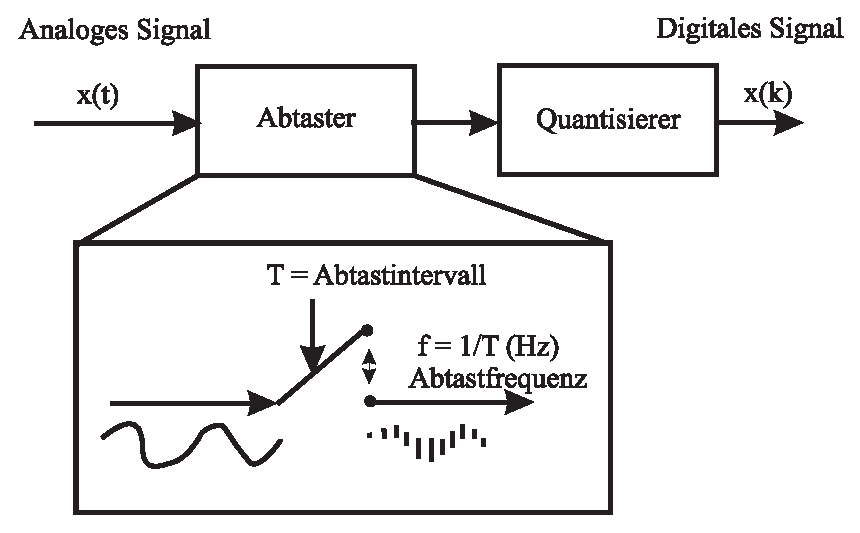
\includegraphics[width = 14cm]{ps/Signalfluss}
\caption{\label{pic:SignalflussAbtastung} Signalfluss zur
Digitalisierung eines analogen Signals.}
\end{center}
\end{figure}


In der DSV geht man in den meisten Fällen implizit davon aus, dass
diese Abtastung in einem regelmäßigen Interval
erfolgt, dass bei Zeitsignalen Abtastinterval $T$ genannt wird
\footnote{Diese Regelmäßigkeit ist aber nicht zwingend, sie vereinfacht nur die weitergehenden Überlegungen.}
(Bei Bildern ist dies die Auflösung).

Die Abtastrate, im weiteren auch mit dem eingedeutschten Begriff Samplingfrequenz $f_s$ bezeichnet,
ist der Kehrwert zum Abtastinterval
\[
    f_s = \frac{1}{T}
\]
und wird in Hertz (Hz) also $1/s$ angegeben.

Die Frage lautet nun, mit welcher Frequenz muss ein Signal abgetastet werden, damit
die digitale Repräsentation dem analogen Original entspricht. Insbesondere,wenn man abschließend
das digitale Signal wieder in ein analoges Signal zurück wandeln will, ist die Frage, welche Frequenz
ist notwendig um eine vollständige Rekonstruktion, also eine verlustlose Diskretisierung,
zu erreichen.

Um dies zu veranschaulichen, sind in der Abbildung \ref{pic:ABtastungErklaerung1}
verschiedene Sinustöne gezeigt, die
bei gleichbleibender Abtastrate abgetastet werden. Es wird deutlich dass, sehr tiefe Frequenzen
besonders gut dargestellt werden (a), je höher die Frequenzen werden, desto weniger Abtastwerte
repräsentieren die analoge Funktion (b,c). Ist die Frequenz des Sinus genau halb so hoch
kann die Funktion gar nicht mehr erkannt werden, da sich eine Konstante ergibt(d).
Erhöht man die Frequenz des Sinus noch weiter entsprechen die Abtastwerte genau den
Abtastwerten einer niedrigeren Frequenz (e,f). Betrachtet man nur die Folge der Abtastwerte
und nicht die Zeitpunkte
des Auftretens\footnote{Diese Information ist nach einer Abtastung nicht mehr vorhanden}, so kommt es
zu Doppeldeutigkeiten. Dieser
Effekt wird {\em Aliasing} genannt.
\begin{figure}[H]
\begin{center}
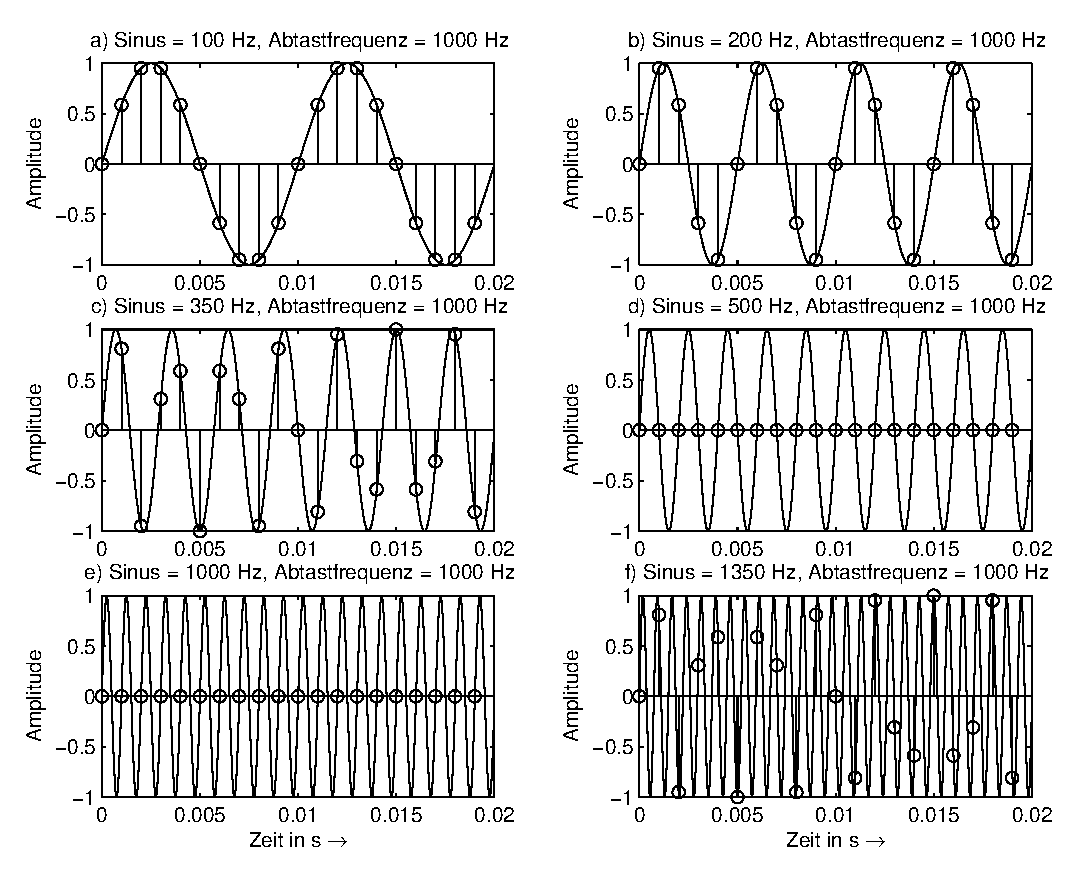
\includegraphics[width = 16cm]{ps/AbtastungErklaerung2}
\caption{\label{pic:ABtastungErklaerung1} Sinusabtastung mit gleichbleibender Abtastrate
für verschiedene Frequenzen.}
\end{center}
\end{figure}

Man kann das Problem aber auch andersherum darstellen. Die Frequenz des Sinus bleibt
gleichbleibend, aber die Abtastrate wird verändert.
Dies ist in Abbildung \ref{pic:ABtastungErklaerung2} gezeigt. Ist die
Abtastrate sehr hoch, kann die Sinusfunktion sehr gut repräsentiert
werden (a). Reduziert man die Abtastfrequenz wird die Anzahl der Samples
die den Sinus repräsentieren immer geringer (b,c). Ist die Abtastfrequenz
genau doppelt so hoch, wie die Frequenz des Sinus, entsteht für diese
Phasenlage ein Nullsignal (d). Es ist also keine Aussage über das Signal mehr möglich.
Erhöht man die Frequenz weiter, so enstehen die schon vorher erwähnten Doppeldeutigkeiten.
\begin{figure}[H]
\begin{center}
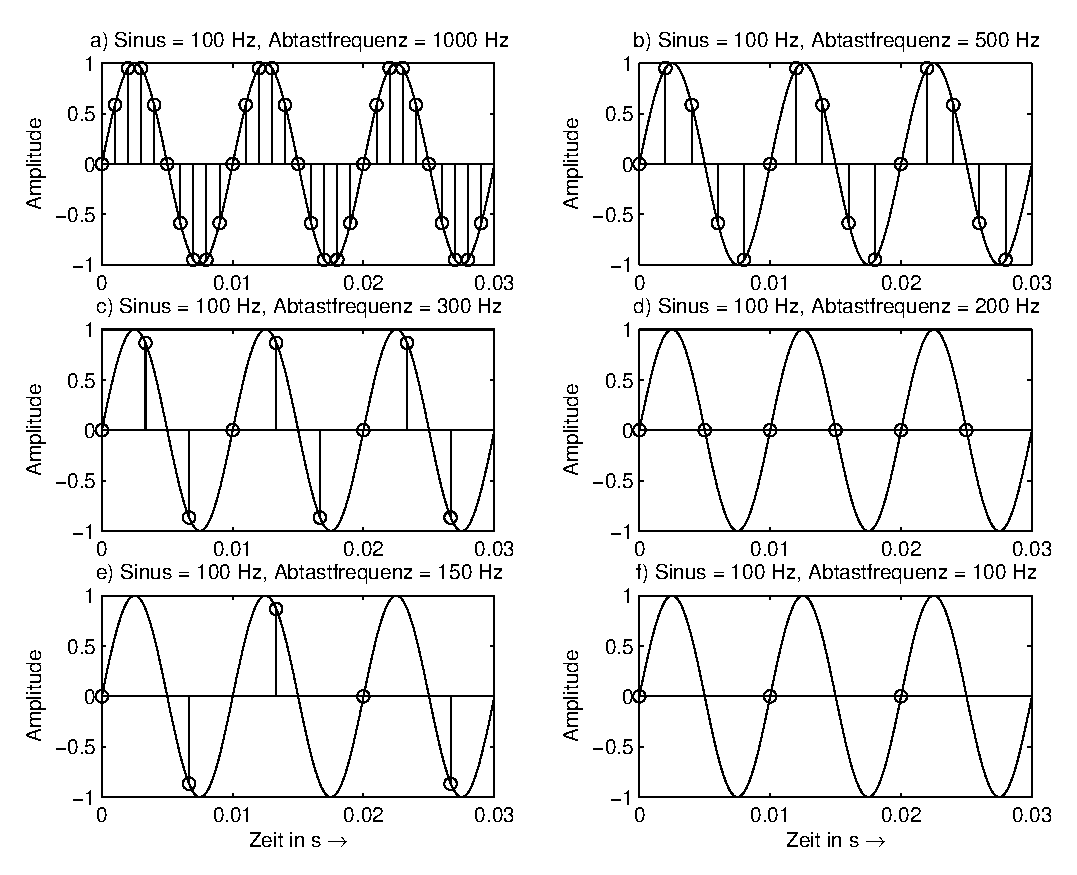
\includegraphics[width = 16cm]{ps/AbtastungErklaerung}
\caption{\label{pic:ABtastungErklaerung2} Sinusabtastung mit unterschiedlichen
Abtastfrequenzen.}
\end{center}
\end{figure}

Um also eine perfekte und eindeutige
Rekonstruktion zu ermöglichen, ist es notwendig, mit wenigstens der doppelten
Frequenz der höchsten im Signal vorkommenden Frequenz abzutasten. Da viele natürliche Signale
keine obere Frequenz haben oder diese so hoch liegt, dass die Abtastung nicht mehr
technisch realisiert werden kann, wird das Eingangssignal einer Abtasteinheit
nach oben begrenzt. Es werden also alle Frequenzen ab einer bestimmten Frequenz aus dem Signal entnommen.
Dieses Prozess bezeichnen wir als Filterung. Das verwendete Filter\footnote{Es heißt
das technische Filter, im Gegensatz zum Kaffeefilter.} wird als Tiefpass-Filter
bezeichnet, da es alle tiefen Frequenzen passieren lässt.

\wichtig{Abtastung ist nur dann eindeutig, wenn das Signal keine Frequenzen enthält, die oberhalb
der halben Abtastfrequenz liegen\footnote{Es wurde bisher nicht gezeigt, dass eine perfekte
Rekonstruktion möglich ist, bzw. dass die wenigen Abtastwerte bei hohen Frequenzen ausreichend sind. Dieser
Tatsache ist hier zunächst zu glauben, da der Beweis nur mit mathematischen Werkzeugen
möglich ist, die zu diesem Zeitpunkt unbekannt sind}
\begin{equation}
f_{max}<\frac{f_s}{2}
\end{equation}
}

Die halbe Samplingfrequenz wird auch als Nyquist-Frequenz bezeichnet.

Um die Abtastung bei einer mathematischen Signalbeschreibung deutlich zu machen, wird
statt der üblichen Beschreibung des analogen  Zeitparameters $t$, die
Index- oder Laufvariable $k$ verwendet\footnote{Lassen Sie sich
nicht verwirren durch andere Bezeichnungen. In der englischsprachigen Literatur wird meist
$n$ als Zeitindex verwendet.}
Eine typisches Zeitsignal $x(t)$ wird also nach der Abtastung zu $x(k)$, wobei
dies eine Abkürzung für $x(kT)$ ist.

\subsection{Quantisierung\label{sec:Quantisierung}}

Der zweite wesentliche Schritt ein digitales Signal zu bekommen ist, die zeitdiskreten Werte
zusätzlich im Wertebereich zu diskretisieren.
Dazu ist es notwendig, eine bestimmte Auflösung und einen bestimmten abzudeckenden Wertebereich festzulegen.
Da wir die Signale digital speichern ist die Auflösung immer in 2er Potenzen angegeben, da
jedes weitere Bit die möglichen Wertestufen um den Faktor 2 erhöht.
Übliche Auflösungen sind 8Bit = 1 Byte, 16Bit = 1 Word oder 32Bit = 1 Long Word.
Damit sind dann 256, 65536 oder $2^{32}$ verschiedene Werte darstellbar.

Zusätzlich muss der Wertebereich nach oben und unten begrenzt sein, da der Wertebereich
von $-\infty  \cdots +\infty$ sonst nicht durch eine begrenzte Anzahl an Stufen aufzulösen ist,
wenn alle Wertestufen den gleichen Abstand haben sollen.

Die eigentliche Werteumwandlung lässt sich am einfachsten anhand von Abbildung
\ref{pic:Quantisierer} zeigen. Auf der x-Achse ist der analoge wertkontinuierliche Eingang
aufgetragen und auf der y-Achse der Ausgang des Diskretisierers, im weiteren Quantisierer
genannt.
\begin{figure}[H]
\begin{center}
\includegraphics[width = 7cm]{ps/Quantisierer}
\caption{\label{pic:Quantisierer} Einfache Quantisierungskennlinie.}
\end{center}
\end{figure}


Diese stufenförmige Funktion wird Quantisierungskennlinie genannt und kann unterschiedlich
aufgebaut sein. In den meisten Fällen sind die Wertestufen alle gleich hoch, man spricht in diesem
Fall auch von einer linearen Quantisierung\footnote{Wir werden auf den Begriff der Linearität noch
kommen und diesen Begriff an dieser Stelle hinterfragen.} Es gibt aber auch andere
Kennlinie, die eine hohe Auflösung im Bereich um Null und bei großen Eingangswerten
eine geringere Auflösung besitzen (Beispiel siehe Abbildung \ref{pic:NonLinearQuant}).
\begin{figure}[H]
\begin{center}
\includegraphics{ps/LogQuant}
\caption{\label{pic:NonLinearQuant} Beispiel einer nicht-linearen
Quantisierungskennlinie.}
\end{center}
\end{figure}

Ein Beispiel hierfür benutzen Sie fast täglich
beim Telefonieren, wo das Signal fast logarithmisch quantisiert wird. Der Vorteil
dieser nicht-gleichförmigen Quantisierung ist die bessere Anpassung an das zu quantisierende
Signal. Als Nachteil erweist sich aber, dass die Signalverarbeitung mit diesen Signalen
sehr viel aufwändiger ist. Deshalb werden diese nicht-gleichförmigen Quantisierer meistens
bei der Speicherung und der Übertragung von Daten verwendet.


Weitere Variationen ergeben sich im Verhalten am Nulldurchgang.
Zum einen kann man das Nullsignal ausschließen oder man weist sehr
kleine Werte alle dem Nullsignal zu (siehe Abbildung
\ref{pic:MidTreadMidRise}). Die letzterer ist die Form die in den
allermeisten Fällen in der Praxis verwendet wird.

\begin{figure}[H]
\begin{center}
\includegraphics{ps/MidRiseMidTread}
\caption{\label{pic:MidTreadMidRise} Quantisierungskennlinie eines
Mid-Tread und eines Mid-Rise Quantisierers. Üblich ist Mid-Tread.}
\end{center}
\end{figure}


Problematisch ist nun aber, dass die benötigte Auflösung bei einer vollständig symmetrischen
Lösung ungerade sein müsste, da die Null weder eine positive noch eine negative Zahl darstellt.
Gleichzeitig muss aber eine 2er Potenz und somit eine gerade Zahl erreicht werden.
Dies wird gelöst, indem die Null zu den positiven Werten gezählt wird. Aus diesem Grund
ergeben sich am Ausgang der meisten Quantisierer
$2^{Bit-1}$ negative Werte, aber nur $2^{Bit-1}-1$ positive Werte. Diese Werte werden
für die Verarbeitung meist normiert angewendet.
Es ergibt sich dann ein Wertebereich von\footnote{Dieser maximale Wert wird auch als 0dbFS bezeichnet. 0dB,
da der Logarithmus von 1= 0 ist und FS für die englische Bezeichnung Full Scale}.
\[
    -1 \leq x \leq 1-\frac{1}{2^{Bit-1}}
\]

Die Frage, welche Auflösung nötig ist, um eine perfekte Rekonstruktion für einen
bestimmten Wertebereich zu ermöglichen ist aber damit noch nicht beantwortet. Das
Problem ist in Abbildung \ref{pic:QuantisierungSinus}
veranschaulicht, die die Quantisierung einer Sinusfunktion mit wenigen Stufen zeigt.

\begin{figure}[H]
\begin{center}
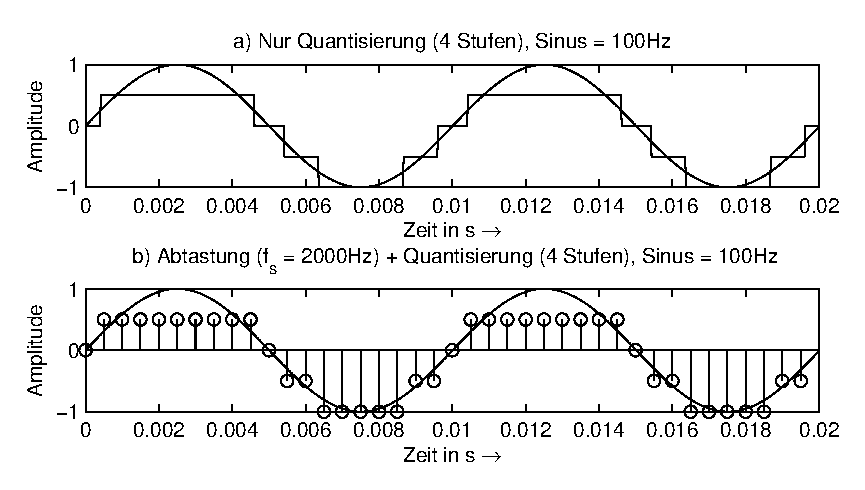
\includegraphics{ps/PlotQuantisierung}
\caption{\label{pic:QuantisierungSinus} Veranschaulichung der Quantisierung
bei einem Sinus als Eingangssignal (Midtread Kennlinie).}
\end{center}
\end{figure}

Es wird deutlich, dass viele unterschiedliche Eingangswerte einem einzigen Ausgangswert
zugewiesen werden (Im Englischen auch als {\em Many--to--One}-Transformation bezeichnet).
Dieser Prozess ist aber immer irreversibel, da aus den quantisierten Werten nicht eindeutig auf die
Originalwerte geschlossen werden kann.

\wichtig{Bei einer Quantisierung kommt es immer zu einem Informationsverlust\footnote{Es kann auch kein Informationsverlust auftreten, wenn das Eingangssignal des Quantisierers auch schon wertdiskret ist.}.}

Die Quantisierung muss also immer so groß gewählt werden, dass sie für den jeweiligen Empfänger angepasst ist. In der Audiologie ist der Empfänger meist das Ohr. Da das Ohr nur einen eingeschränkten Dynamikbereich wahrnimmt, reichen 16Bit, wie sie bei der CD verwendet werden, meistens aus. Die entstandenen Verzerrungen sind für ungeübte Ohren unhörbar und werden als Rauschen wahrgenommen. Dies gilt zumindest wenn die Auflösung bezogen auf die Amplitude des Signals ausreicht.

\section{Einige Elementarsignale}
In der Einführung wurden einige Beispiele für Signale genannt, die meist aus einer direkten Beobachtung der Natur folgten. Für den weiteren Verlauf ist es aber notwendig auf Signale zurückgreifen zu können, die mathematisch beschreibbar sind, um weitere Berechnungen zu ermöglichen

\subsection{Determinierte Signale}
Vollständig beschreibare Signale werden als deterministisch bezeichnet. Ihr
Signalverlauf ist zu jedem Zeitpunkt eindeutig angegeben. Wir unterscheiden
zusätzlich bei den deterministischen Signalen ob eine Periodizität vorliegt, oder nicht.
\subsubsection{Periodische Signale}
Periodische Signale zeichnen sich durch eine Wiederholung ihrer Signalform
innerhalb eines bestimmten Periodendauer $P$ aus. Es gilt:
\begin{equation}\label{eq:PeriodischSignale}
    x(t) = x(t+nP) \quad \Mit \quad n\in\mathbb{Z}
\end{equation}
Einige periodische Signale sind:
\begin{itemize}
\item{{\bf Sinus:}
Die vollständige Beschreibung des Sinustones ist durch
\begin{equation}
y(t) = \underbrace{a}_{\mbox{Amplitude}} \sin(\underbrace{\omega}_{\mbox{Kreisfrequenz}} t +
\underbrace{\varphi}_{\mbox{Phase}})
\end{equation}
bzw. häufiger durch
\begin{equation}
y(t) = \underbrace{a}_{\mbox{Amplitude}} \cos(\underbrace{\omega}_{\mbox{Kreisfrequenz}} t +
\underbrace{\varphi}_{\mbox{Phase}})
\end{equation}
gegeben\footnote{Der Cosinus ist für viele Anwendungen leichter zu berechnen, \zB bei der Fourier-Transformation, da sich ein rein reelles Spektrum ergibt.}. Die Kreisfrequenz $\omega$ setzt sich dabei aus $\omega =
2 \pi f$ zusammen, wobei $f$ die eigentliche Frequenz in Hertz
$1Hz = 1 s^{-1}$ darstellt. Sie gibt an, wie viele Perioden einer
Schwingung in einer Sekunde Signal vorhanden sind, daher $s^{-1}$
= pro Sekunde als Maßeinheit.
Um die anderen Parameter etwas zu verdeutlichen, sind in den Abbildungen \ref{pic:SinusAmplitude}
- \ref{pic:SinusPhase} verschiedene Sinustöne bei variierenden Parametern gezeigt.
\begin{figure}[htb]
\begin{minipage}{5cm}
%\begin{figure}[htb]
\includegraphics [width = 5cm]{ps/SinusAmplitude}
\caption{\label{pic:SinusAmplitude} Veränderung der Amplitude}
%\end{figure}
\end{minipage}
\begin{minipage}{5cm}
%\begin{figure}[htb]
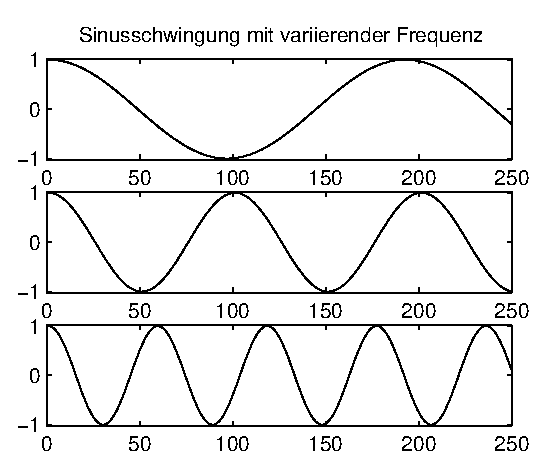
\includegraphics [width = 5cm]{ps/SinusFrequenz}
\caption{\label{pic:Veranschaulichung Schwingung}Veränderung der Frequenz}
%\end{figure}
\end{minipage}
\begin{minipage}{5cm}
%\begin{figure}[htb]
\includegraphics [width = 5cm]{ps/SinusPhase}
\caption{\label{pic:SinusPhase}Veränderung der Anfangsphase}
%\end{figure}
\end{minipage}
\end{figure}
}

Die Erzeugung einer diskreten Folge, die einen Cosinus repräsentiert kann durch
\begin{equation}\label{eq:DiscreteSinus}
    y(k) = a \cos\left(2\pi k \frac{f_0}{f_s}  + \varphi_0 \right)
\end{equation}
erzeugt werden. Bei dieser Darstellung ist die Abkürzung für
\[
    kT = \frac{k}{f_s}
\]
leicht erkennbar \footnote{Üblicherweise wird die Cosinus-Fkt als Elemetarsignal genutzt und nicht der Sinus, da dieser für spätere Betrachtungen einige positive Eigenschaften aufweist}.


\item{{\bf Dreieck:} Ein periodisches Dreieckssignal zu beschreiben, kann auf zwei Arten erfolgen.
Eine sehr einfache Beschreibung erfolgt über eine abschnittsweise Definition. Eine Periode der
Dreiecksschwingung ist gegeben durch
\begin{equation}\label{eq:DreieckAbschnitt}
x_{1D}(t) = \bigg\{ \begin{array}{lcc}
1-\left|\frac{2t}{L}\right| & & -L \leq t \leq L\\
0 & & \mbox{sonst}
\end{array}
\end{equation}
Die Periodizität wird abschließend durch
\begin{equation}
x(t+n2L) = x(t)
\end{equation}
für $n \in\mathbb{Z}$ erzeugt.
\begin{figure}[h]
\begin{center}
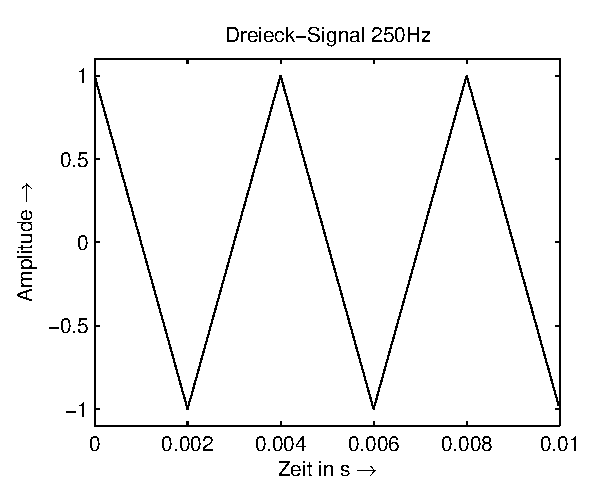
\includegraphics[width = 8cm]{ps/Dreieck}
\caption{\label{pic:DreieckFunktion} Ausschnitt eines Dreiecksignals.}
\end{center}
\end{figure}

Eine weitere Möglichkeit periodische Signale auszudrücken, ergibt sich aus dem Fourier-Theorem. Es besagt,
dass sich alle periodischen Signale auf eine Summe von Sinussignalen zurückführen lassen. Die zerlegten
komplexen Signale lassen sich dann durch eine sog. Fourier-Reihe beschreiben.
Für das Dreieckssignal ist diese Fourier-Reihe durch
\begin{equation}\label{eq:DreieckFourier}
y(t) = \frac{8}{\pi^2}\left(\sin(\omega t) - \frac{1}{3^2} \sin(3\omega t) + \frac{1}{5^2} \sin(5 \omega t) - \cdots\right)
\end{equation} 
oder
\begin{equation}\label{eq:DreieckFourier2}
y(t) = \frac{8}{\pi^2}\left(\cos(\omega t) + \frac{1}{3^2} \cos(3\omega t) + \frac{1}{5^2} \cos(5 \omega t) + \cdots\right)
\end{equation} 
gegeben. Hierbei handelt es sich also um eine unendliche Reihe von Sinustönen, die nur ungeradzahlige
Vielfache der Grundfrequenz\footnote{Treten in einer komplexen Schwingung ganzzahlige (ob
geradzahlig oder ungeradzahlig ist nicht relevant) Vielfache der Grundfrequenz auf, so werden diese
Vielfachen auch Harmonische der Grundfrequenz genannt. Die erste Harmonische ist dabei die Grundfrequenz
selbst.} sind, wobei die Amplitude mit dem Quadrat des Vielfachen abnimmt. Für eine digitale Realisierung
stellt sich hier nun ein Problem ein. Würden wir die abschnittsweise Definition aus
Gleichung \ref{eq:DreieckAbschnitt} direkt in einem digitalen System implementieren, so würde dieses
Signal nach Gleichung \ref{eq:DreieckFourier} auch Frequenzen oberhalb der halben Abtastfrequenz
aufweisen. Ein so direkt erzeugtes Dreieckssignal besitzt deshalb immer Aliasing-Anteile, die aber
in einigen Fällen durch die sehr geringe Amplitude vernachlässigbar sind.
\tbd{Diskrete Dreieck Schwingung}
}
\item{
{\bf Rechteck:} Für das Rechtecksignal funktionieren ebenfalls die beiden Methoden.
Wir können eine abschnittsweise Definition verwenden:
\begin{equation}\label{eq:RechteckAbschnitt}
x_{1R}(t) = \bigg\{ \begin{array}{lcc}
-1 & & -L \leq t < 0\\
1 & &0 \leq t < L
\end{array}
\end{equation}
Die Periodizität wird wieder durch
\begin{equation}\label{eq:Periodizitaet}
x(t+n2L) = x_{1R}(t)
\end{equation}
für $n \in \mathbb{Z}$ erreicht.

Die Fourier-Reihe für ein periodisches Rechtecksignal ist
\begin{equation}\label{eq:RechteckFourier}
y(t) = \frac{4}{\pi}\left(\sin(\omega t) + \frac{1}{3} \sin(3\omega t) + \frac{1}{5} \sin(5 \omega t) + \cdots\right).
\end{equation}
Auch hier treten nur ungeradzahlige Harmonische auf, die aber im Vergleich zu der Dreiecksschwingung
nur mit dem Vielfachen und nicht mit dem Quadrat abnehmen. Dies bedeutet, dass die Aliasing-Problematik
noch ausgeprägter ist.

Eine dritte Methode, die eine besonders einfache Implementierung ermöglicht, ergibt sich aus
der signum-Funktion, die jeweils das Vorzeichen angibt.
\begin{equation}
sign(x) = \left\{ \begin{array}{lcc}
-1 & & x<0\\
0 & & 0\\
1 & & x>0
\end{array} \right.
\end{equation}
Eine Rechteckfunktion kann nun sehr einfach durch das Vorzeichen der Sinusfunktion angegeben werden:
\begin{equation}\label{eq:EasyRechteck}
x(t) = sign(\sin(\omega t));
\end{equation}
bzw. in diskreter Form durch
\begin{equation}\label{eq:EasyRechteckDiskret}
x(k) = sign(\sin\left(2\pi k \frac{f_0}{f_s}\right));
\end{equation}

\begin{figure}[h]
\begin{center}
\includegraphics[width = 8cm]{ps/Rechteck}
\caption{\label{pic:RechteckFunktion} Ausschnitt eines Rechtecksignals, erzeugt mit \ref{eq:EasyRechteck}.}
\end{center}
\end{figure}



}
\item{
{\bf Sägezahn:} Eine weitere etwas speziellere Schwingung stellt die Sägezahnschwingung dar, die
besonders häufig bei Synthesizern als Quellensignal zur Erzeugung von Tönen verwendet wird.
Es sind wieder zwei Definitionen möglich.
Die abschnittsweise Definition ergibt sich zu
\begin{equation}
x(t) =\bigg\{ \begin{array}{lcc}
-1+ t/L & &  0 \leq t < 2L\\
0 & & \mbox{sonst}
\end{array}
\end{equation}
Die Periode wird erneut durch Gleichung \ref{eq:Periodizitaet} erzeugt.
Interessant ist die Fourier-Reihenentwicklung:
\begin{equation}
y(t) = \frac{2}{\pi}\left(\sin(\omega t) - \frac{1}{2} \sin(2\omega t) + \frac{1}{3} \sin(3\omega t)
- \frac{1}{4} \sin(4\omega t) + \frac{1}{5} \sin(5 \omega t) - \cdots\right).
\end{equation}
Bei der Sägezahnschwingung treten alle ganzzahligen Harmonischen auf und der Abfall der Amplitude ist gering.
Dieser hohe Anteil an Harmonischen ist auch die Begründung
für den Einsatz bei der elektronischen Klangerzeugung, da sich ein vollerer Klang ergibt, der anschließend manipuliert werden kann.
\begin{figure}[h]
\begin{center}
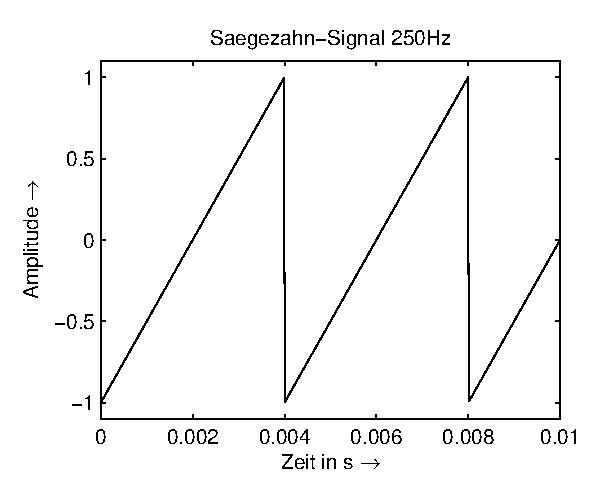
\includegraphics[width = 8cm]{ps/Saegezahn}
\caption{\label{pic:SaegezahnFunktion} Ausschnitt eines Sägezahnsignals.}
\end{center}
\end{figure}
\tbd{Diskreter Sägezahn}
}
\end{itemize}

\subsubsection{Impulssignale}
Eine weitere wichtige Klasse der determinierten Signale stellen die Impulssignale dar:
\begin{itemize}
    \item{{\bf Delta-Impuls\footnote{Auch als zeitdiskreter Dirac-Impuls bekannt}:}
    Der Delta-Impuls ist die wichtigste digitale Impulsfolge, sie wird auch
    als Kronecker-Delta bezeichnet und ist definiert durch
    \begin{equation}
    \delta(k) = \bigg\{ \begin{array}{lcc}
       1 & & k = 0\\
        0  & & \mbox{sonst}
    \end{array}
    \end{equation}
    Aus der Definition folgt
    \begin{equation}
        x(k) \delta(k) = x(0),
    \end{equation}
    was als Siebeigenschaft des Delta-Impulses bekannt ist.
\begin{figure}[h]
\begin{center}
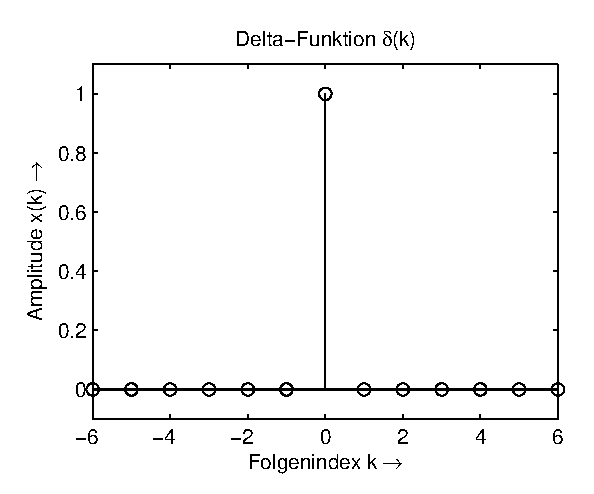
\includegraphics[width = 8cm]{ps/DeltaFunktion}
\caption{\label{pic:DeltaFunktion} Delta-Folge.}
\end{center}
\end{figure}

}
\item{{\bf Sprungfolge:} Die Sprungfolge ist neben dem Delta-Impuls eine weitere sehr wichtige
    Folge zur Beurteilung digitaler Systeme.
    \begin{equation}\label{eq:Def:Sprungfolge}
        \gamma(k) = \bigg\{ \begin{array}{lcc}
        1 & & k \geq 0\\
        0 & & \mbox{sonst}
        \end{array}
    \end{equation}
\begin{figure}[h]
\begin{center}
\includegraphics[width = 8cm]{ps/SprungFunktion}
\caption{\label{pic:SprungFunktion} Sprung-Folge.}
\end{center}
\end{figure}
}
\item{{\bf Exponential Impuls:} Die Exponentialfolge ist durch
    \begin{equation}
        x(t) = A e^{\alpha t}
    \end{equation}
    gegeben, wobei $\alpha$ die Dämpfungskonstante angibt und nur für $\alpha < 1$ eine stabile Funktion darstellt.
    Häufig wird aber statt $\alpha$ direkt anzugeben eine sog. Zeitkonstante $\tau = -1 / \alpha$ angegeben.
    Diese beschreibt die Zeit, in der die Funktion auf ca. $37$\% von $A$ abgeklungen ist (siehe
    Abbildung \ref{pic:ExpImpulse}) und das Integral der Exponentialfunktion dem äquivalenten Rechteck bis $\tau$ entspricht.
    \begin{figure}[h]
    \begin{center}
    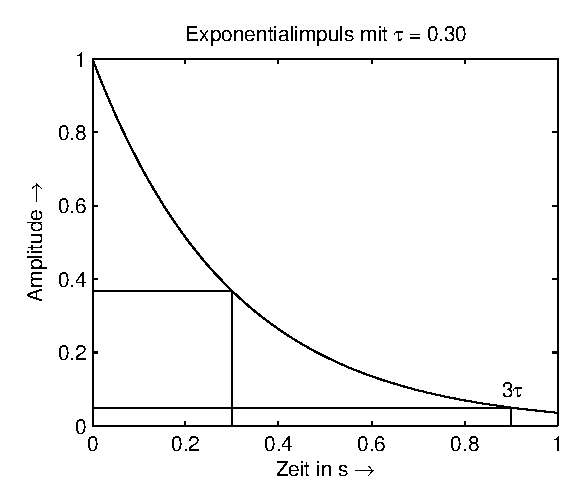
\includegraphics[width = 8cm]{ps/ExpImpulse}
    \caption{\label{pic:ExpImpulse} Exponential Impuls für $\tau = 0.3$s. Eingezeichnet ist
    zusätzlich der $\approx 5$\% Punkt, der sich bei $3\tau$ ergibt.}
    \end{center}
    \end{figure}
    
    
    In der diskreten Form ist die Wertefolge durch

    \begin{equation}\label{eq:ExpImpulseDiskret}
        x(k) = A e^{\alpha k/f_s}
    \end{equation}
    gegeben. Abbildung \ref{pic:ExpImpulseDiskret} zeigt einen diskreten Exponentialimpuls mit
    den Parametern $A = 1, f_s = 2$kHz und $\tau = 3$ms.

    \begin{figure}[h]
    \begin{center}
    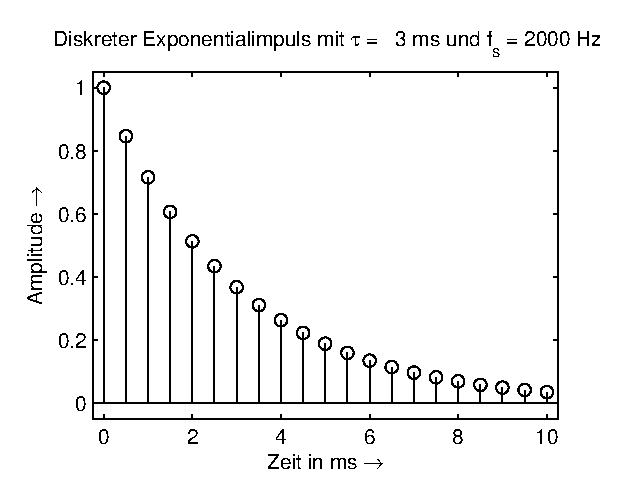
\includegraphics[width = 8cm]{ps/ExpImpulseDiskret}
    \caption{\label{pic:ExpImpulseDiskret} Diskreter Exponential Impuls für
    $\tau = 3$ms.}
    \end{center}
    \end{figure}
    
    Eine alternative Beschreibung ist die Definition als Exponentialfolge
    \[
        x(k) = \alpha_2^{k} \gamma(k)
    \]
    mit
    \[
        \alpha_2 = 1-\frac{1}{\tau f_s}
    \]
    
    }
    \item{{\bf si-Signal:} Die si-Funktion ist zunächst analog definiert und wird in
    nachfolgenden Abschnitten
    benötigt, um \zB die Abtastung genauer zu erläutern.
    \begin{equation}
    si(t) = \frac{\sin t}{t}
    \end{equation}
    bzw.\ häufig wird auch
   \begin{equation}
    sinc(t) = \frac{\sin \pi t}{\pi t}
    \end{equation}
    definiert. In Matlab ist nur \verb/sinc/ implementiert.
    Der Impuls ist in beiden Fällen eine abklingende Sinusschwingung. Der Unterschied ist die
    x-Achsen-Skalierung.
    \begin{figure}[H]
    \begin{center}
    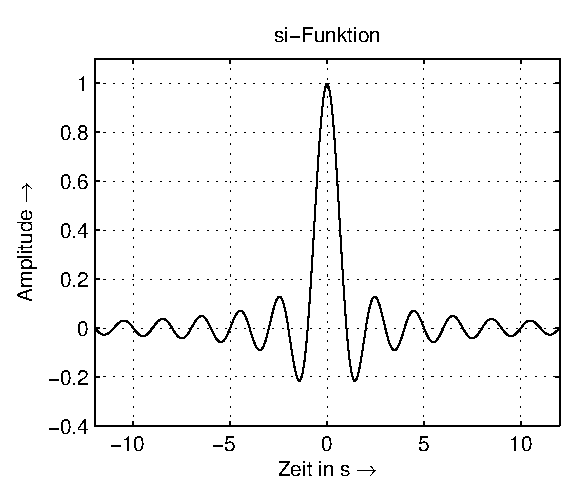
\includegraphics[width = 8cm]{ps/SiFunktion}
    \caption{\label{pic:SiFunktion} Sinc-Impuls auf den Definitionsbereich $-12 \leq t \leq 12$ beschränkt.}
    \end{center}
    \end{figure}
    Für die diskrete si-Folge, nutzen wir die Definition des diskreten Sinus
    aus Gleichung \ref{eq:DiscreteSinus}, mit der Amplitude 1 und einem Anfangswinkel von $\pi/2$.
    Somit wird die Cosinus-Funktion zum Sinus. Es ergibt sich also für die diskrete si-Folge
    \begin{equation}\label{eq:DEF:DiscreteSi}
        si(k) = \frac{sin \left(2\pi k\frac{f_0}{f_s} \right)}{2\pi k\frac{f_0}{f_s}}
    \end{equation}
    Abbildung \ref{pic:SiFunktionDiskret} zeigt eine diskrete si-Folge. Die 100Hz Schwingung
    bei einer Abtastrate von $f_s = 1000$ Hz ist gut an den Nulldurchgängen zu erkennen.
    \begin{figure}[H]
    \begin{center}
    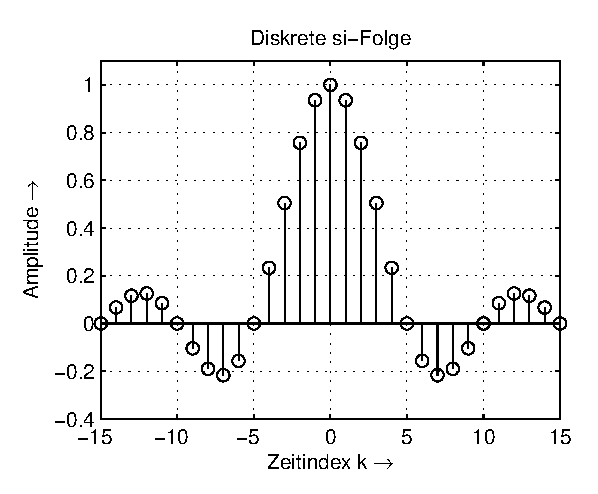
\includegraphics[width = 8cm]{ps/SiFunktionDiskret}
    \caption{\label{pic:SiFunktionDiskret} Si-Folge im Bereich $-15 \leq k \leq 15$ für $f_0 = 100$ Hz und
    $f_s = 1000$ Hz.}
    \end{center}
    \end{figure}

    }
    \item{{\bf Dirac-Impuls:} Der analoge Dirac-Impuls $\Dirac{t}$,
kann nicht direkt als Funktion definiert werden. Statt dessen
erfolgt die Definition über das Integral
\begin{equation}\label{eq:Def:Dirac-Impulse}
   \int\limits_{-\infty}^{\infty}f(t)\Dirac{t} dt = f(0),
\end{equation}
wobei $f(t)$ eine beliebige stetige und differenzierbare Funktion
ist. Die Aussage der Gleichung \ref{eq:Def:Dirac-Impulse} ist, dass der Dirac-Impulse aus
einem Signal nur und ausschließlich den Wert des Signals zum
Zeitpunkt Null herausfiltert. Dies wird auch als Sieb-Eigenschaft
bezeichnet und entspricht der besonderen Eigenschaft des
Delta-Impulses für diskrete Signale. Da keine direkte Definition
möglich ist, spricht man beim Dirac-Impulse von einer
verallgemeinerten Funktion. Diese besondere Klasse ist auch unter
dem Begriff Distributionen bekannt. Durch die Definition als unendlich kurzen
und unendlichen hohen Impuls wird deutlich, dass dieser Impuls nicht
realisierbar ist, sondern eine reine theoretische Konstruktion darstellt, die
sich aber als sehr nützlich Werkzeug zum Berechnen bestimmter Probleme heraus gestellt hat.

Weitere Eigenschaften des Dirac-Impulses sind:
\begin{equation}\label{eq:Eigenschaft1:Dirac}
    \Dirac{t} = 0 \fuer t \neq 0
\end{equation}
Außerdem gilt
\begin{equation}\label{eq:Eigenschaft2:Dirac}
     \int\limits_{-\infty}^{\infty}\Dirac{t} dt = 1
\end{equation}
Aus der Definition und den beiden Eigenschaften können weitere
wichtige Eigenschaften abgeleitet werden. So gilt für den zeitlich
verschobenen Dirac-Impuls:
\begin{equation}\label{eq:Eigenschaft3:Dirac}
    x(t)\Dirac{t-t_0} = x(t_0)\Dirac{t-t_0}
\end{equation}
und
\begin{equation}\label{eq:Eigenschaft4:Dirac}
   \int\limits_{-\infty}^{\infty}x(t)\Dirac{t-t_0} dt = x(t_0),
\end{equation}
Für einen zeitlich skalierten Dirac-Impuls gilt:
\begin{equation}\label{eq:EigenschaftSkalierung:Dirac}
    \Dirac{\alpha t} = \frac{1}{|\alpha|}\Dirac{t} \quad
    \mbox{bzw.}\quad \int\limits_{-\infty}^{\infty}\Dirac{\alpha t} dt =
    \frac{1}{|\alpha|}
\end{equation}
    }
\end{itemize}

\subsection{stochastische Signale \label{sec:stochastEinfuehrung}}
Eine sehr wichtige Klasse an Signalen sind die stochastischen oder
auch rauschförmigen Signale. Sie zeichnen sich dadurch aus, dass
man den Signalverlauf nicht direkt vorhersagen kann. Trotzdem
ist es möglich bestimmte Eigenschaften rauschförmiger Signale
zu beschreiben. Einige grundlegende Beschreibungsgrößen sind:

\begin{itemize}
\item{{\bf Mittelwert:} Die Schätzung\footnote{Schätzungen werden häufig durch $\hat{\cdot}$ markiert}
des Mittelwert ist definiert als die Summe aller
Werte geteilt durch die Anzahl $N$ der gemittelten Werte
\begin{equation}
    \hat{\mu} = \bar{x} = \frac{1}{N} \sum_{k = 1}^{N} x(k)
\end{equation}
}
\item{{\bf Varianz:} Die Schätzung der Varianz ist die mittlere quadratische Abweichung aller Werte vom Mittelwert.
Die Wurzel aus der Varianz wird Standardabweichung $\sigma$ genannt. Deshalb definieren wir die
Varianz durch $\sigma^2$
\begin{equation}
    \hat{\sigma}^2 = \frac{1}{N-1} \sum_{k = 1}^{N} (x(k)-\mu)^2
\end{equation}
}

\item{{\bf Amplitudenverteilung:} Die Amplitudenverteilung gibt an, wie oft die einzelne Amplitudenwerte
im Signal vorkommen. Dies kann häufig mathematisch ausgedrückt werden. Liegt eine
bestimmte Datenfolge vor, wird statt dessen das Histogramm berechnet. Das Histogramm unterteilt den
Eingangsbereich der Amplituden in gleichbleibende Abschnitte und zählt dann aus, wie oft
die Datenfolge Werte in diesem Bereich hat. In Matlab wird dies durch den Befehl \Matlab{hist}
realisiert. Zwei sehr oft vorkommende Amplitudenverteilungen bei Rauschsignalen sind die
gleichförmige Verteilung und die gaussförmige Verteilung. Bei der gleichförmigen Verteilung
kommen in einem definierten Wertebereich alle Amplitudenwerte gleich oft vor. In Matlab
werden Rauschsignale mit dieser Eigenschaft durch den Befehl \Matlab{rand} erzeugt.
Die Verteilung bei der Gauss-Verteilung hat dagegen eine Glockenform. Bestimmte Wertebereiche kommen
also häufiger vor als andere. Die Beschreibung ist mathematisch durch
\begin{equation}
 p(x) = \frac{1}{\sigma \sqrt{2\pi}} e^{-\frac{(x(k)-\mu)^2}{2\sigma^2}}
\end{equation}
gegeben. Wir sehen, dass die beiden Größen Mittelwert und Varianz hier als formgebende Größen
verwendet werden. In Matlab können solche Verteilungen mit dem Befehl \Matlab{normrnd} erzeugt werden.
Gaussverteiltes Rauschen mit der Varianz $\sigma^2= 1$ und dem Mittelvert $\mu= 0$ erzeugt der
Befehl \Matlab{randn}.
Abbildung \ref{pic:Verteilungen} zeigt einige Beispiele mit unterschiedlichen Parametern.
\begin{figure}[H]
\begin{center}
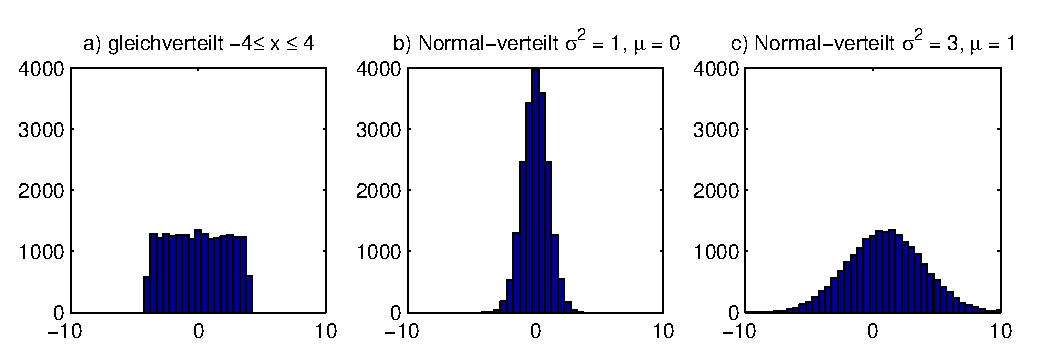
\includegraphics[width = 16cm]{ps/Verteilungen}
\caption{\label{pic:Verteilungen} Beispiele für unterschiedliche Amplitudenverteilungen, wobei
für alle drei Bilder 20000 Datenwerte verwendet wurden.}
\end{center}
\end{figure}
Die Gauss-Verteilung wird auch als Normal-Verteilung bezeichnet. Sie hat eine
große Bedeutung, da bei einer unendlichen Mittelung vieler unabhängiger, gleichverteilter
Verteilungen immer eine Normal-Verteilung am Ende herauskommt. Diese Tatsache wird
zentraler Grenzwertsatz genannt.
}
\end{itemize}

\section{Weitere Eigenschaften von Signalen}
\subsection{Kausalität}
Kausalität bedeutet, dass eine Wirkung immer eine zeitlich vorhergehende Ursache haben muss.
Für Signale heißt diese Eigenschaft, dass keine Signalanteile vor $t = 0$ existieren dürfen.
Alle Anteile mit $t<0$ oder $k < 0$ sind nicht-kausale Anteile des Signals (siehe Abbildung
\ref{pic:KausalErklaerung}).

\begin{figure}[h]
\begin{center}
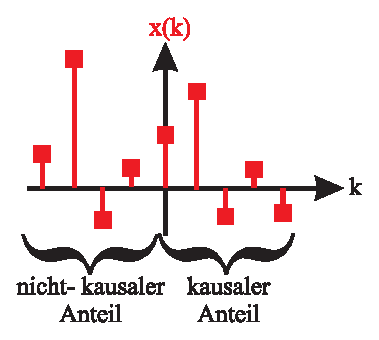
\includegraphics{ps/KausalErklaerung}
\caption{\label{pic:KausalErklaerung} Erklärung zum Begriff der Kausalität bei Signalen.}
\end{center}
\end{figure}

\subsection{Energie und Leistung \label{sec:EnergUndLeistung}}
Es muss zwischen Energie- und Leistungssignalen unterschieden werden
\begin{itemize}
\item{Die Energie eines diskreten Signals ist durch
\begin{equation}
    E_x = \sum_{k = -\infty}^{\infty} |x(k)|^2
\end{equation}
gegeben. Aufgrund dieser Definition ist deutlich, dass alle periodischen Signale
eine Energie $E_x=\infty$ haben.

Für analoge Signale gilt:
\begin{equation}
    E_x = \int_{-\infty}^{\infty} |x(t)|^2 dt
\end{equation}
}
\item{Die Definition der mittleren Leistung wird im diskreten Fall durch
\begin{equation}
    P_x =\lim_{n\rightarrow \infty} \frac{1}{2n+1} \sum_{k = -n}^{n} |x(k)|^2
\end{equation}
und für analoge Signale durch
\begin{equation}
    P_x =\lim_{T\rightarrow \infty} \frac{1}{T} \int_{-\frac{T}{2}}^{\frac{T}{2}} |x(t)|^2 dt
\end{equation}
angegeben. Von einem Leistungssignal spricht man, wenn $0 < P_x < \infty$ gilt.
Periodische Signale sind also Leistungssignale. Weiterhin kann bei periodischen Signalen
zur Berechnung der Leistung
nur eine Periode betrachtet werden, was zu einer vereinfachten Berechnung führt.
Die Leistung aller Energiesignale ist null, da der Nenner im Bruch vor der Summe im Grenzfall $\infty$ wird.
}
\end{itemize}

\begin{example} Wie groß ist die Leistung eines Sinussignal mit der Amplitude $A$.
\begin{eqnarray}
    P_x & = & \lim_{T\rightarrow \infty} \frac{1}{T} \int_{-\frac{T}{2}}^{\frac{T}{2}} |A sin(t)|^2 dt\\
    & = & \frac{1}{2\pi} \int_{-\pi}^{\pi} A^2 sin^2(t) dt\\
    & = & \frac{A^2}{2\pi} \left( \frac{1}{2}t - \frac{1}{4} \sin (2t) \right)\Bigg]_{-\pi}^{\pi}\\
    & = & \frac{A^2}{2\pi} \left( \frac{1}{2}t - \frac{1}{4} \sin (2t)\right)\Bigg]_{-\pi}^{\pi} \\
    & = & \frac{A^2}{2\pi} \left( \frac{1}{2} \pi + \frac{1}{2} \pi \right) \\
    & = & \frac{A^2}{2}
\end{eqnarray}
\end{example}

\subsection{Zeitliche Verschiebung}
Häufig ist es notwendig Signale zeitlich verschoben zu definieren, um bestimmte Aspekte oder
das Zusammenspiel zweier Signale zu verdeutlichen. Dies wird erreicht, indem die unabhängige Zeitvariable
$t$ bzw. $k$ um einen festen Faktor $t_0$ bzw. $k_0$ verschoben wird. Eine Verzögerung erfolgt über ein
negatives Vorzeichen, also $t-t_0$ bzw. $k-k_0$. Eine positive zeitliche Verschiebung durch $t+t_0$ bzw.
$k+k_0$ (siehe Abbildung \ref{pic:VerschobenesRechteck}).

Bei diskreten Signale ist zu beachten, dass immer eine Verschiebung
um ganzzahlige Vielfache des Abtastintervals vorgenommen werden $k_0 = nT$ mit
$n \in \mathbb{Z}$
\footnote{Es ist auch möglich
nichtganzzahlige Verzögerungen zu realisieren, aber dies wird meist nur in sehr
speziellen Fällen benötigt. Das Stichwort hierzu lautet {\em Fractional Delay Filter}}.

\begin{figure}[h]
\begin{center}
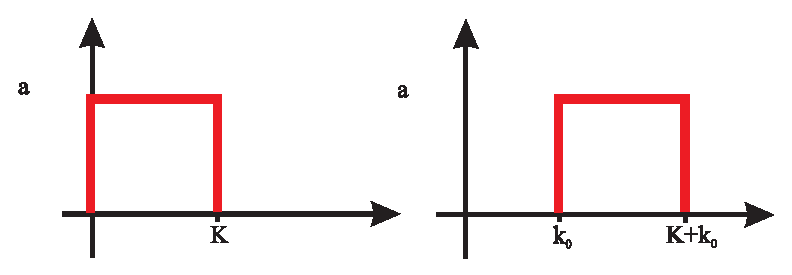
\includegraphics[width = 8cm]{ps/ZeitlicheVerschiebung}
\caption{\label{pic:VerschobenesRechteck} Veranschaulichung einer zeitlichen Verschiebung (Verzögerung)
um $k_0$.}
\end{center}
\end{figure}

\subsection{Darstellung diskreter Signale als Delta-Impulsfolgen}
\tbd{Alle digitalen Signale lassen sich als Summe von gewichteten und verschobenen Delta-Impulsen darstellen $x(k) = \sum x_{\kappa} \delta(k-\kappa)$}

\compileif{bBook}
{
\section{Darstellung und Generierung von Signalen in Matlab}
Für diesen Abschnitt siehe Matlab-Script. Ist hier nur aufgeführt als ein ToDo Punkt.

\subsection{Rauschsignale}
\subsection{determinierte Signale}
\subsubsection{Impulssignale}
\subsubsection{Periodische Signale}

\subsection{Darstellung}
\tbd{Plot, Stem. Hist}
}

\section{Übungen}
\subsection{Wiederholung des Stoffes und einfache Rechenaufgaben}
\begin{enumerate}
    \item Klassifizieren Sie folgende Signale anhand der im Skript angegeben Merkmale:
    \begin{enumerate}
        \item $si(t)$
        \item Das digitale (SP-DIF) und analoge Signal eines CD-Players
        \item Ein DVD Film
        \item Vielleicht ihr Beispiel
    \end{enumerate}
    \item Was ist die Grundvoraussetzung für eine erfolgreiche Digitalisierung?
    \item Warum verliert man Informationen bei der Digitalisierung?
    \item Warum lassen sich Funktionen mit Knickstellen (Bsp: Dreieck) nicht wirklich digitalisieren?
    \item Welches ist die höchste Harmonische einer aliasingfreien Dreieckschwingung mit der Grundfrequenz
    $f = 440$ Hz, bei einer Abtastrate von $f_s = 48000$ Hz?
    \item Zeigen Sie, dass $si(0) = 1$ ist!
    \item Zeichnen Sie $x(k) = 2\delta(k+2) - 0.5\delta(k-1) + 3\delta(k-2)$!
\end{enumerate}

\subsection{Aufgaben (Auf Klausurniveau)}
\begin{enumerate}
    \item Wie hoch ist die Leistung eines mittelwertfreien Dreieckssignals mit der Amplitude A?
    \item
    \item
\end{enumerate}

\compileif{bBook}{
\subsection{Matlab-Aufgaben}
\begin{enumerate}
    \item Programmieren Sie eine Funktion, die einen Mid-Tread Quantisierer mit einer Auflösung von
    4 Bit realisiert. Versuchen Sie so allgemein zu programmieren, dass Sie jederzeit die Auflösung
    ändern können.
    \item Programmieren Sie einen Rechtecksignal-Generator in Matlab, mit und ohne Aliasing.
    \item Erzeugen Sie eine Funktion die eine Delta-Impulsfolge mit vordefinierter Länge (Angabe
    in Sekunden und $f_s$) zurück gibt.
\end{enumerate}
}

\subsection{Transfer-Leistung}
\tbd{Fraglich ob hier möglich}
%
\compileif{bZusammenfassung}
{
\section{Zusammenfassung}
Die wichtigen Erkenntnisse aus diesem Kapitel sind:
\begin{itemize}
    \item Die Umwandlung analoger in digitale Signale erfolgt in zwei Schritten:
    \begin{itemize}
        \item Abtastung: verlustlos möglich, wenn gilt $f_{max} < f_s/2$ (Abtasttheorem)
        \item Quantisierung: verlustbehaftet
    \end{itemize}
    \item Mathematische Betrachtungen erfolgen meist mit diskreten Signalen (Annahme unendliche Genauigkeit)
    \item Signale lassen sich klassifizieren:
    \begin{itemize}
        \item Kanalanzahl
        \item Dimensionalität
        \item usw.
    \end{itemize}
    \item Es gibt Energie- und Leistungssignale:
    \begin{itemize}
        \item Energiesignale haben keine Leistung
        \item Leistungssignale haben eine unendliche Energie
     \end{itemize}
     \item Signale, die nicht stetig und/oder differenzierbar (\zB Rechteck, Dreieck)
     sind sind nicht bandbegrenzt und können
     deshalb nicht verlustlos diskretisiert werden.
    \item Dirac und Delta-Funktion stellen wichtige Elementarsignale dar.
\end{itemize}
}
